\documentclass{standalone}
\usepackage{tikz}
\usepackage{pgfplots}
\usetikzlibrary{arrows.meta}

\begin{document}
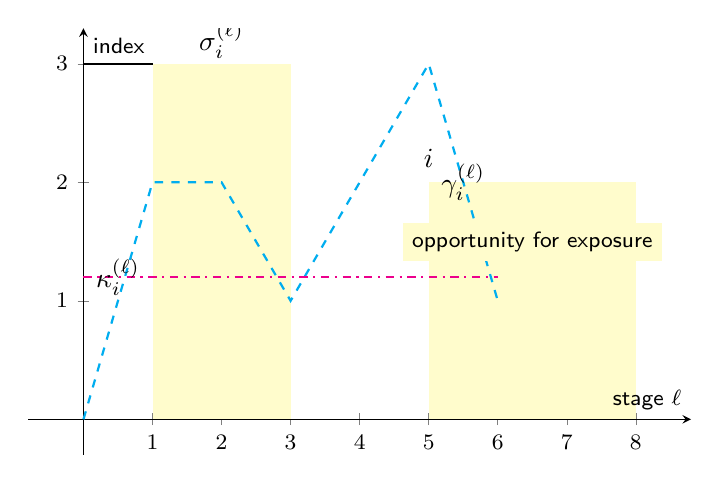
\begin{tikzpicture}
  \begin{axis}[
      axis lines=middle, enlargelimits, xlabel={stage $\ell$}, ylabel={index},
      xtick distance=1, ytick distance=1,
      every axis label/.style={font=\footnotesize\sffamily},
      every tick label/.style={font=\footnotesize\sffamily},
      width=10cm, height=7cm
    ]

    % 阴影区域
    \addplot[domain=1:3, samples=2, draw=none, fill=yellow!20] {3} \closedcycle;
    \addplot[domain=5:8, samples=2, draw=none, fill=yellow!20] {2} \closedcycle;

    % 阶梯线
    \addplot[thick, cyan, dashed] coordinates {(0,0) (1,2) (2,2) (3,1) (5,3) (6,1)};
    \addplot[thick, magenta, dash dot] coordinates {(0,1.2) (6,1.2)};
    \addplot[thick, black] coordinates {(0,3) (1,3)};

    % 节点标记
    \node at (axis cs: 2,3.2) {\(\sigma_i^{(\ell)}\)};
    \node at (axis cs: 5,2.2) {\(i\)};
    \node[fill=yellow!20, font=\footnotesize\sffamily, anchor=mid] at (axis cs: 6.5,1.5) {opportunity for exposure};
    \node at (axis cs: 0.5,1.2) {\(\kappa_i^{(\ell)}\)};
    \node at (axis cs: 5.5,2) {\(\gamma_i^{(\ell)}\)};
    
  \end{axis}
\end{tikzpicture}
\end{document}